% Chapter Template

\chapter{Literature Review}\doublespacing % Main chapter title

\label{Chapter2} % Change X to a consecutive number; for referencing this chapter elsewhere, use \ref{ChapterX}

\lhead{Chapter II. \emph{Literature Review}} % 

\section{Introduction}

Malware analysis and privilege escalation attacks have become critical areas of research in modern cybersecurity. 
With the increasing number of cyber-attacks targeting operating systems such as Microsoft Windows, advanced 
techniques have been developed to detect, analyze, and mitigate malicious software.

Windows operating systems rely on several internal components such as dynamic link libraries (DLLs), system calls, 
kernel services, and access control mechanisms. Libraries such as \textbf{Kernel32.dll}, \textbf{Ntdll.dll}, and 
\textbf{User32.dll} provide an interface between user applications and the Windows kernel.

Attackers exploit vulnerabilities in these components to gain elevated privileges or execute malicious code. 
Privilege escalation attacks allow attackers to obtain administrative or kernel-level access and perform 
unauthorized operations within the system.

These attacks are generally categorized into two types:

\begin{itemize}
\item Horizontal Privilege Escalation
\item Vertical Privilege Escalation
\end{itemize}

Recent research focuses on advanced techniques such as dynamic malware analysis, behavioral monitoring, 
and direct system call execution techniques such as the \textbf{Hell's Gate technique}.

---


\section{Windows Architecture}

Understanding Windows internal architecture is essential for malware analysis.

\begin{figure}[H]
\centering
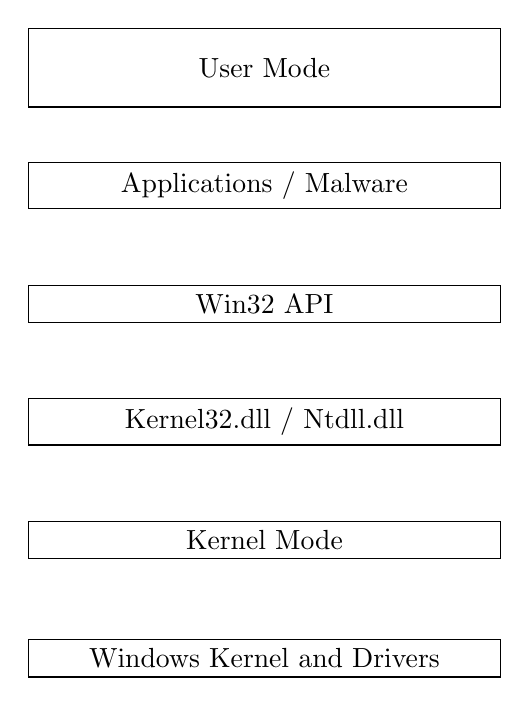
\begin{tikzpicture}[node distance=1.5cm]

\node (user) [rectangle, draw, minimum width=6cm, minimum height=1cm] {User Mode};
\node (apps) [rectangle, draw, below of=user, minimum width=6cm] {Applications / Malware};
\node (api) [rectangle, draw, below of=apps, minimum width=6cm] {Win32 API};
\node (dll) [rectangle, draw, below of=api, minimum width=6cm] {Kernel32.dll / Ntdll.dll};

\node (kernel) [rectangle, draw, below of=dll, minimum width=6cm] {Kernel Mode};
\node (kmod) [rectangle, draw, below of=kernel, minimum width=6cm] {Windows Kernel and Drivers};

\end{tikzpicture}
\caption{Windows User Mode and Kernel Mode Architecture}
\end{figure}

Applications interact with the operating system using the Win32 API. These APIs eventually trigger system calls 
that transfer execution from user mode to kernel mode.

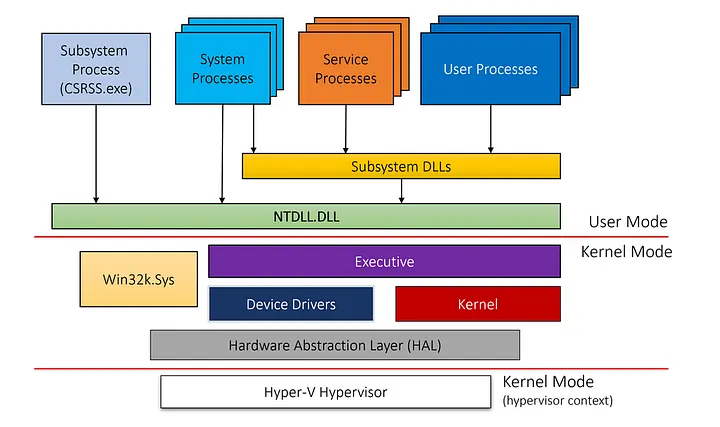
\includegraphics[width=\linewidth]{Images/Windows_Architecture.png}

Applications interact with the Windows operating system using \textbf{Win32 APIs}, which are implemented in libraries such as:

\begin{itemize}
    \item \texttt{kernel32.dll}
    \item \texttt{ntdll.dll}
    \item \texttt{advapi32.dll}
\end{itemize}

These APIs eventually invoke \textbf{system calls} that transition execution from \textit{user mode} to \textit{kernel mode}.

\section{System Calls and NTDLL}

The \textbf{NTDLL.dll} library plays a crucial role in Windows internals because it provides the interface for 
executing system calls. Each user-mode process implicitly links against NTDLL, which contains wrappers that 
transition execution to kernel mode.

A typical system call implementation follows this pattern:

\begin{lstlisting}
mov r10, rcx
mov eax, syscall_number
syscall
ret
\end{lstlisting}

The \texttt{syscall} instruction transfers execution to the Windows kernel where privileged operations are performed.

\section{Hell's Gate Technique}

The Hell's Gate technique is a modern malware technique that dynamically retrieves system call numbers from 
NTDLL instead of relying on static API calls.

Traditional malware relies on functions such as:

\begin{verbatim}
LoadLibrary()
GetProcAddress()
\end{verbatim}

However, these APIs are frequently monitored by security solutions such as antivirus and endpoint detection systems.

Hell's Gate bypasses this monitoring by directly resolving system calls from memory.

\begin{figure}[H]
\centering
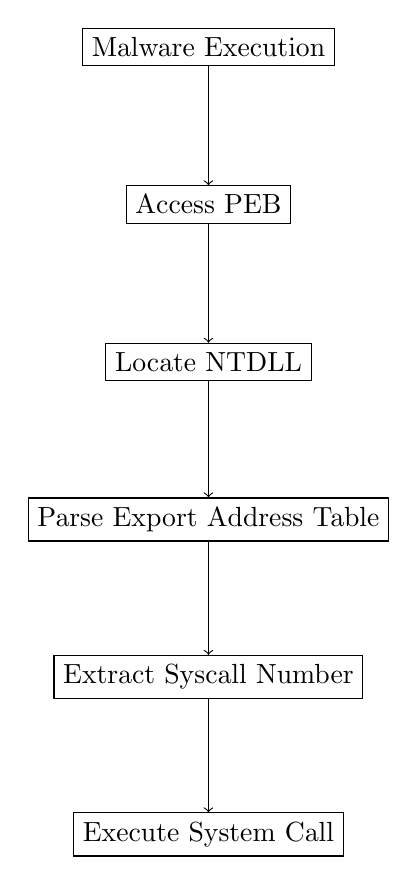
\begin{tikzpicture}[node distance=2cm]

\node (mal) [rectangle, draw] {Malware Execution};
\node (peb) [rectangle, draw, below of=mal] {Access PEB};
\node (ntdll) [rectangle, draw, below of=peb] {Locate NTDLL};
\node (export) [rectangle, draw, below of=ntdll] {Parse Export Address Table};
\node (syscall) [rectangle, draw, below of=export] {Extract Syscall Number};
\node (kernel) [rectangle, draw, below of=syscall] {Execute System Call};

\draw[->] (mal) -- (peb);
\draw[->] (peb) -- (ntdll);
\draw[->] (ntdll) -- (export);
\draw[->] (export) -- (syscall);
\draw[->] (syscall) -- (kernel);

\end{tikzpicture}
\caption{Hell's Gate System Call Resolution Process}
\end{figure}

This technique allows malware to evade many detection mechanisms by avoiding monitored API functions.

---
\subsection{Hell's Gate Technique for Direct System Call Resolution}

The Hell's Gate technique is a modern malware evasion technique that allows programs to dynamically resolve 
and execute Windows system calls without relying on standard API functions. Instead of invoking Windows API 
functions such as \texttt{LoadLibrary} or \texttt{GetProcAddress}, Hell's Gate directly retrieves system call 
numbers from the \texttt{NTDLL.dll} module at runtime.

The main objective of the Hell's Gate technique is to locate and traverse the Export Address Table (EAT) of 
\texttt{NTDLL.dll} in memory and dynamically extract the system call numbers associated with internal NT 
functions such as \texttt{NtCreateMutant}, \texttt{NtAllocateVirtualMemory}, and others.

\subsubsection{Export Address Table Traversal}

To locate system calls dynamically, the technique traverses the Portable Executable (PE) structure of 
\texttt{NTDLL.dll}. The process involves several steps:

\begin{enumerate}
\item Retrieve the base address of the loaded module.
\item Access the \texttt{\_IMAGE\_DOS\_HEADER} and verify the \texttt{IMAGE\_DOS\_SIGNATURE}.
\item Traverse the \texttt{\_IMAGE\_NT\_HEADERS}, \texttt{\_IMAGE\_FILE\_HEADER}, and \texttt{\_IMAGE\_OPTIONAL\_HEADER}.
\item Locate the Export Address Table inside the \texttt{\_IMAGE\_DATA\_DIRECTORY}.
\item Typecast the structure to \texttt{\_IMAGE\_EXPORT\_DIRECTORY}.
\end{enumerate}

The following code illustrates how the Export Address Table can be accessed from memory:

\begin{lstlisting}
PPEB Peb = (PPEB)__readgsqword(0x60);
PLDR_MODULE pLoadModule;
PBYTE ImageBase;

pLoadModule = (PLDR_MODULE)((PBYTE)
Peb->LoaderData->InMemoryOrderModuleList.Flink->Flink - 16);

ImageBase = (PBYTE)pLoadModule->BaseAddress;

\end{lstlisting}

    



After retrieving the base address, the PE structures are parsed sequentially:

\begin{lstlisting}
    PIMAGE_DOS_HEADER Dos = (PIMAGE_DOS_HEADER)ImageBase;

if (Dos->e_magic != IMAGE_DOS_SIGNATURE)
    return 1;

PIMAGE_NT_HEADERS Nt =
(PIMAGE_NT_HEADERS)((PBYTE)Dos + Dos->e_lfanew);

PIMAGE_FILE_HEADER File =
(PIMAGE_FILE_HEADER)(ImageBase +
(Dos->e_lfanew + sizeof(DWORD)));

PIMAGE_OPTIONAL_HEADER Optional =
(PIMAGE_OPTIONAL_HEADER)((PBYTE)File +
sizeof(IMAGE_FILE_HEADER));

PIMAGE_EXPORT_DIRECTORY ExportTable =
(PIMAGE_EXPORT_DIRECTORY)
(ImageBase + Optional->DataDirectory[0].VirtualAddress);
\end{lstlisting}



Once the Export Address Table is reached, it contains several important arrays:

\begin{itemize}
\item FunctionNameAddressArray – contains function names
\item FunctionOrdinalAddressArray – indexes for functions
\item FunctionAddressArray – addresses of exported functions
\end{itemize}

These arrays allow traversal of exported functions within \texttt{NTDLL.dll}.

\subsubsection{System Call Extraction}

Each NT system function follows a common instruction pattern that loads the system call 
number into the \texttt{EAX} register before executing the \texttt{syscall} instruction.

Example disassembly:

\begin{lstlisting}
    mov r10, rcx
mov eax, 0B3h
syscall
ret
\end{lstlisting}



Here, the system call number (\texttt{0xB3}) is loaded into the \texttt{EAX} register and 
executed using the \texttt{syscall} instruction.

The system call identifier can be extracted from the function's instruction bytes:

\begin{lstlisting}
    db (ntdll!NtCreateMutant + 0x4) L 2
00007fff`b040c3d4 b3 00
\end{lstlisting}



The syscall value is calculated as:

\begin{lstlisting}
    (0x00 << 8) | 0xb3 = 179
\end{lstlisting}



\subsubsection{Executing System Calls Using Hell's Gate}

Once the syscall number is extracted, Hell's Gate uses a small assembly routine 
to dynamically execute the syscall.

\begin{lstlisting}
    .data
wSystemCall DWORD 000h

.code
HellsGate PROC
    mov wSystemCall, ecx
    ret
HellsGate ENDP

HellDescent PROC
    mov r10, rcx
    mov eax, wSystemCall
    syscall
    ret
HellDescent ENDP
\end{lstlisting}



The \texttt{HellsGate} function stores the syscall number, while \texttt{HellDescent} 
executes the syscall instruction.

Example usage:

\begin{lstlisting}
    WORD syscall = 0x00b3;

HellsGate(syscall);

HANDLE hMutant = INVALID_HANDLE_VALUE;

NTSTATUS st =
HellDescent(&hMutant, MUTANT_ALL_ACCESS, NULL, TRUE);
\end{lstlisting}


This approach allows malware or red-team tools to bypass traditional API monitoring 
mechanisms and execute system calls directly, thereby evading detection mechanisms 
implemented by security products such as antivirus or EDR systems.

\section{Privilege Escalation Techniques}

Privilege escalation attacks occur when attackers gain higher permissions than originally assigned to them.

Common privilege escalation methods include:

\begin{itemize}
\item DLL Hijacking
\item Token Impersonation
\item Unquoted Service Path Exploitation
\item SAM Hash Extraction
\end{itemize}

---

\section{SAM Hash Extraction}

The \textbf{Security Account Manager (SAM)} database stores user authentication information in Windows systems.

The SAM file is located at:

\begin{verbatim}
C:\Windows\System32\config\SAM
\end{verbatim}

Attackers extract password hashes from the SAM file using tools such as \textbf{secretsdump}.

\begin{verbatim}
secretsdump.py -sam SAM -security SECURITY -system SYSTEM local
\end{verbatim}

Extracted hashes are then cracked using password recovery tools such as \textbf{Hashcat}.

---

\section{Privilege Escalation Attack Workflow}

\begin{figure}[H]
\centering
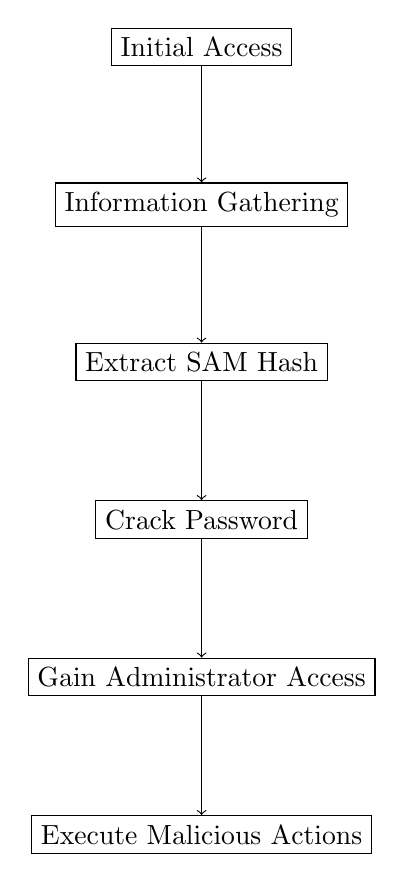
\begin{tikzpicture}[node distance=2cm]

\node (init) [rectangle, draw] {Initial Access};
\node (info) [rectangle, draw, below of=init] {Information Gathering};
\node (hash) [rectangle, draw, below of=info] {Extract SAM Hash};
\node (crack) [rectangle, draw, below of=hash] {Crack Password};
\node (admin) [rectangle, draw, below of=crack] {Gain Administrator Access};
\node (attack) [rectangle, draw, below of=admin] {Execute Malicious Actions};

\draw[->] (init) -- (info);
\draw[->] (info) -- (hash);
\draw[->] (hash) -- (crack);
\draw[->] (crack) -- (admin);
\draw[->] (admin) -- (attack);

\end{tikzpicture}
\caption{Privilege Escalation Attack Workflow}
\end{figure}

---

\section{Research Gap}

Despite advancements in malware detection techniques, many security systems still rely on signature-based detection 
and API monitoring. Modern malware techniques such as direct system calls and dynamic syscall resolution allow 
attackers to bypass these detection mechanisms.

Therefore, new approaches are required to analyze malware behavior more effectively. Visualization-based systems 
such as the proposed \textbf{Malviz} framework aim to represent malware activity in a graphical form, enabling 
security analysts to better understand complex attack patterns.

---

\section{Summary}

This chapter reviewed existing literature on malware analysis, Windows internals, system call mechanisms, and 
privilege escalation techniques. Modern attack methods such as Hell's Gate demonstrate how malware can evade 
traditional detection mechanisms. These techniques highlight the need for improved analysis tools capable of 
visualizing and interpreting malicious system behavior.







